% answers.tex —— 2009 年·普通高等学校招生考试·重庆卷·理科 · 参考答案与详细解析片段
% 由 tools/generate_projects.py 依来源总账自 2009/2009_数学真题_重庆理_试题.md + 2009/2009_数学真题_重庆理_解析正文.md + 2009/2009_数学真题_重庆理_答案要点.md 生成，勿手改（改源 MD 后重跑）


\begin{gktip}
固定候选 PDF 仅含题面，无答案、解析和评分标准，原页亦未标分值；以下为非官方编者独立推导，官方答案字段为空。分数、根号、上下标与两幅图均以 600 dpi 原页复核。第 20 题准线原页印作 $x=\frac{4\sqrt3}3$，但与 $C(0,-\sqrt3)$、$D(0,\sqrt3)$、$e=\frac{\sqrt3}2$ 及公开答案册的 $|MC|\cdot|MD|$ 最大值 $4$ 矛盾；按唯一自洽的 $y=\frac{4\sqrt3}3$（椭圆 $\frac{x^2}1+\frac{y^2}4=1$）求解，并登记 \texttt{ISSUE-1516}。
\end{gktip}

\begin{answer}
\gksolhead{1}{}

\textbf{题目}：

直线 $y=x+1$ 与圆 $x^2+y^2=1$ 的位置关系是（　）

（A）相切

（B）相交但直线不过圆心

（C）直线过圆心

（D）相离

\Needspace{4\baselineskip}
\textbf{解析}

直线 $x-y+1=0$ 到圆心 $(0,0)$ 的距离为 $\dfrac1{\sqrt2}<1$，故相交；原点不满足 $x-y+1=0$，故直线不过圆心。

\gkanswer{答案：B。}

\end{answer}
\begin{answer}
\gksolhead{2}{}

\textbf{题目}：

已知复数 $z$ 的实部为 $-1$，虚部为 $2$，则 $\dfrac{5i}{z}=$（　）

（A）$2-i$

（B）$2+i$

（C）$-2-i$

（D）$-2+i$

\Needspace{4\baselineskip}
\textbf{解析}

\Needspace{5\baselineskip}
$z=-1+2i$，

\nopagebreak[4]
\[\frac{5i}{z}=\frac{5i}{-1+2i}
=\frac{5i(-1-2i)}{(-1)^2+2^2}
=\frac{10-5i}{5}=2-i.\]

\gkanswer{答案：A。}

\end{answer}
\begin{answer}
\gksolhead{3}{}

\textbf{题目}：

$\left(x^2+\dfrac2x\right)^8$ 的展开式中 $x^4$ 的系数是（　）

（A）$16$

（B）$70$

（C）$560$

（D）$1120$

\Needspace{4\baselineskip}
\textbf{解析}

\nopagebreak[4]
\[\left(x^2+\frac2x\right)^8\]
\Needspace{5\baselineskip}
的通项为 $\mathrm C_8^k(x^2)^{8-k}\left(\frac2x\right)^k=\mathrm C_8^k2^kx^{16-3k}$。令 $16-3k=4$，得 $k=4$，系数

\nopagebreak[4]
\[\mathrm C_8^4\cdot2^4=70\times16=1120.\]

\gkanswer{答案：D。}

\end{answer}
\begin{answer}
\gksolhead{4}{}

\textbf{题目}：

已知 $|\boldsymbol a|=1$，$|\boldsymbol b|=6$，$\boldsymbol a\cdot(\boldsymbol b-\boldsymbol a)=2$，则向量 $\boldsymbol a$ 与 $\boldsymbol b$ 的夹角是（　）

（A）$\dfrac\pi6$

（B）$\dfrac\pi4$

（C）$\dfrac\pi3$

（D）$\dfrac\pi2$

\Needspace{4\baselineskip}
\textbf{解析}

\Needspace{5\baselineskip}
由 $\boldsymbol a\cdot(\boldsymbol b-\boldsymbol a)=2$ 得 $\boldsymbol a\cdot\boldsymbol b-|\boldsymbol a|^2=2$，故 $\boldsymbol a\cdot\boldsymbol b=3$。于是

\nopagebreak[4]
\[\cos\theta=\frac{\boldsymbol a\cdot\boldsymbol b}{|\boldsymbol a||\boldsymbol b|}
=\frac3{1\times6}=\frac12,\]

$\theta=\dfrac\pi3$。

\gkanswer{答案：C。}

\end{answer}
\begin{answer}
\gksolhead{5}{}

\textbf{题目}：

不等式 $|x+3|-|x-1|\leqslant a^2-3a$ 对任意实数 $x$ 恒成立，则实数 $a$ 的取值范围为（　）

（A）$(-\infty,-1]\cup[4,+\infty)$

（B）$(-\infty,-2]\cup[5,+\infty)$

（C）$[1,2]$

（D）$(-\infty,1]\cup[2,+\infty)$

\Needspace{4\baselineskip}
\textbf{解析}

\Needspace{5\baselineskip}
由三角不等式，

\nopagebreak[4]
\[|x+3|-|x-1|\leqslant|(x+3)-(x-1)|=4,\]

\Needspace{5\baselineskip}
且 $x\geqslant1$ 时可取到 $4$。故须

\nopagebreak[4]
\[4\leqslant a^2-3a,\qquad a^2-3a-4\geqslant0,\qquad (a-4)(a+1)\geqslant0,\]

即 $a\leqslant-1$ 或 $a\geqslant4$。

\gkanswer{答案：A。}

\end{answer}
\begin{answer}
\gksolhead{6}{}

\textbf{题目}：

锅中煮有芝麻馅汤圆 $6$ 个，花生馅汤圆 $5$ 个，豆沙馅汤圆 $4$ 个，这三种汤圆的外部特征完全相同．从中任意舀取 $4$ 个汤圆，则每种汤圆都至少取到 $1$ 个的概率为（　）

（A）$\dfrac8{91}$

（B）$\dfrac{25}{91}$

（C）$\dfrac{48}{91}$

（D）$\dfrac{60}{91}$

\Needspace{4\baselineskip}
\textbf{解析}

\Needspace{5\baselineskip}
总数 $\mathrm C_{15}^4=1365$。每种至少 $1$ 个，只能是 $2,1,1$ 分配：

\nopagebreak[4]
\[3\times\left(\mathrm C_6^2\cdot5\cdot4+\mathrm C_5^2\cdot6\cdot4+\mathrm C_4^2\cdot6\cdot5\right)\]

\Needspace{5\baselineskip}
更直接地，三类分别为 $2,1,1$ 的和：

\nopagebreak[4]
\[\mathrm C_6^2\cdot5\cdot4+\mathrm C_5^2\cdot6\cdot4+\mathrm C_4^2\cdot6\cdot5
=300+240+180=720.\]

\Needspace{5\baselineskip}
概率

\nopagebreak[4]
\[\frac{720}{1365}=\frac{48}{91}.\]

\gkanswer{答案：C。}

\end{answer}
\begin{answer}
\gksolhead{7}{}

\textbf{题目}：

设 $\triangle ABC$ 的三个内角 $A$，$B$，$C$，向量 $\boldsymbol m=(\sqrt3\sin A,\sin B)$，$\boldsymbol n=(\cos B,\sqrt3\cos A)$，若 $\boldsymbol m\cdot\boldsymbol n=1+\cos(A+B)$，则 $C=$（　）

（A）$\dfrac\pi6$

（B）$\dfrac\pi3$

（C）$\dfrac{2\pi}3$

（D）$\dfrac{5\pi}6$

\Needspace{4\baselineskip}
\textbf{解析}

\nopagebreak[4]
\[\boldsymbol m\cdot\boldsymbol n
=\sqrt3\sin A\cos B+\sqrt3\sin B\cos A
=\sqrt3\sin(A+B)=\sqrt3\sin C.\]

\Needspace{5\baselineskip}
又 $1+\cos(A+B)=1-\cos C$，故

\nopagebreak[4]
\[\sqrt3\sin C=1-\cos C,\qquad 2\sin\left(C+\frac\pi6\right)=1.\]

由 $0<C<\pi$，得 $C+\dfrac\pi6=\dfrac{5\pi}6$，$C=\dfrac{2\pi}3$。

\gkanswer{答案：C。}

\end{answer}
\begin{answer}
\gksolhead{8}{}

\textbf{题目}：

已知 $\lim\limits_{x\to\infty}\left(\dfrac{2x^2}{x+1}-ax-b\right)=2$，其中 $a,b\in\mathbf R$，则 $a-b$ 的值为（　）

（A）$-6$

（B）$-2$

（C）$2$

（D）$6$

\Needspace{4\baselineskip}
\textbf{解析}

\nopagebreak[4]
\[\frac{2x^2}{x+1}=2x-2+\frac2{x+1},\]

\Needspace{5\baselineskip}
故

\nopagebreak[4]
\[\frac{2x^2}{x+1}-ax-b=(2-a)x-(2+b)+\frac2{x+1}.\]

极限为 $2$，须 $2-a=0$，$-(2+b)=2$，即 $a=2$，$b=-4$，$a-b=6$。

\gkanswer{答案：D。}

\end{answer}
\begin{answer}
\gksolhead{9}{}

\textbf{题目}：

已知二面角 $\alpha-l-\beta$ 的大小为 $50^\circ$，$P$ 为空间中任意一点，则过点 $P$ 且与平面 $\alpha$ 和平面 $\beta$ 所成的角都是 $25^\circ$ 的直线的条数为（　）

（A）$2$

（B）$3$

（C）$4$

（D）$5$

\Needspace{4\baselineskip}
\textbf{解析}

\Needspace{5\baselineskip}
设两平面交线为 $y$ 轴，法向量分别为 $(0,0,1)$ 与 $(\sin50^\circ,0,\cos50^\circ)$。与两平面成 $25^\circ$ 的直线方向 $\boldsymbol u=(x,y,z)$ 满足

\nopagebreak[4]
\[|z|=\sin25^\circ,\qquad |x\sin50^\circ+z\cos50^\circ|=\sin25^\circ.\]

分别取 $z=\pm\sin25^\circ$，各得一个 $y=0$ 的解与两个 $y\neq0$ 的解；按直线不区分方向合并，共 $3$ 条。

\gkanswer{答案：B。}

\end{answer}
\begin{answer}
\gksolhead{10}{}

\textbf{题目}：

\Needspace{5\baselineskip}
已知以 $T=4$ 为周期的函数

\nopagebreak[4]
\[f(x)=\begin{cases}m\sqrt{1-x^2},&x\in(-1,1],\\ 1-|x-2|,&x\in(1,3],\end{cases}\]

其中 $m>0$．若方程 $3f(x)=x$ 恰有 $5$ 个实数解，则 $m$ 的取值范围为（　）

（A）$\left(\dfrac{\sqrt{15}}3,\dfrac83\right)$

（B）$\left(\dfrac{\sqrt{15}}3,\sqrt7\right)$

（C）$\left(\dfrac43,\dfrac83\right)$

（D）$\left(\dfrac43,\sqrt7\right)$

\Needspace{4\baselineskip}
\textbf{解析}

在 $[-1,3]$ 上，$3f(x)=x$ 恒有 $3$ 个解：半圆支一个，$x\in(1,2]$ 与 $x\in[2,3]$ 各一个。要在全 R 上恰有 $5$ 个解，需下一周期 $[3,7]$ 的半圆支恰有 $2$ 个解。

\Needspace{5\baselineskip}
该支方程 $3m\sqrt{1-(x-4)^2}=x$，平方得

\nopagebreak[4]
\[(9m^2+1)(x-4)^2+8(x-4)+(16-9m^2)=0.\]

\Needspace{5\baselineskip}
有两解的条件为判别式

\nopagebreak[4]
\[324m^2\left(m^2-\frac53\right)>0,\]

即 $m>\dfrac{\sqrt{15}}3$。

\Needspace{5\baselineskip}
再下一周期 $[7,11]$ 开始出现解的条件为 $m\geqslant\dfrac83$（半圆支最高点 $x=8$ 处 $3m=8$）。故恰有 $5$ 解当

\nopagebreak[4]
\[\frac{\sqrt{15}}3<m<\frac83.\]

\gkanswer{答案：A。}

\end{answer}
\begin{answer}
\gksolhead{11}{}

\textbf{题目}：

若 $A=\{x\in\mathbf R\mid |x|<3\}$，$B=\{x\in\mathbf R\mid 2^x>1\}$，则 $A\cap B=$ $\underline{\qquad}$．

\Needspace{4\baselineskip}
\textbf{解析}

$A=(-3,3)$，$B=(0,+\infty)$，故 $A\cap B=(0,3)$。

\gkanswer{答案：$(0,3)$。}

\end{answer}
\begin{answer}
\gksolhead{12}{}

\textbf{题目}：

若 $f(x)=\dfrac1{2^x-1}+a$ 是奇函数，则 $a=$ $\underline{\qquad}$．

\Needspace{4\baselineskip}
\textbf{解析}

\Needspace{5\baselineskip}
$f$ 为奇函数，故 $f(x)+f(-x)=0$：

\nopagebreak[4]
\[\frac1{2^x-1}+a+\frac1{2^{-x}-1}+a=0.\]

\Needspace{5\baselineskip}
而 $\dfrac1{2^{-x}-1}=-\dfrac{2^x}{2^x-1}$，故前两项之和为 $-1$，

\nopagebreak[4]
\[-1+2a=0,\qquad a=\frac12.\]

\gkanswer{答案：$\dfrac12$。}

\end{answer}
\begin{answer}
\gksolhead{13}{}

\textbf{题目}：

将 $4$ 名大学生分配到 $3$ 个乡镇去当村官，每个乡镇至少一名，则不同的分配方案有$\underline{\qquad}$种．（用数字作答）

\Needspace{4\baselineskip}
\textbf{解析}

\Needspace{5\baselineskip}
分配人数为 $2,1,1$。选接收两人的乡镇 $3$ 种，选两人 $\mathrm C_4^2=6$ 种，余下两人分配 $2!=2$ 种：

\nopagebreak[4]
\[3\times6\times2=36.\]

\gkanswer{答案：$36$。}

\end{answer}
\begin{answer}
\gksolhead{14}{}

\textbf{题目}：

设 $a_1=2$，$a_{n+1}=\dfrac2{a_n+1}$，$b_n=\dfrac{a_n+2}{a_n-1}$，$n\in\mathbf N^*$，则数列 $\{b_n\}$ 的通项 $b_n=$ $\underline{\qquad}$．

\Needspace{4\baselineskip}
\textbf{解析}

\nopagebreak[4]
\[b_{n+1}=\frac{a_{n+1}+2}{a_{n+1}-1}
=\frac{\frac2{a_n+1}+2}{\frac2{a_n+1}-1}
=\frac{2(a_n+2)}{1-a_n}=-2b_n.\]

$b_1=\dfrac{2+2}{2-1}=4$，故 $b_n=4(-2)^{n-1}=(-1)^{n-1}2^{n+1}$。

\gkanswer{答案：$(-1)^{n-1}2^{n+1}$。}

\end{answer}
\begin{answer}
\gksolhead{15}{}

\textbf{题目}：

已知双曲线 $\dfrac{x^2}{a^2}-\dfrac{y^2}{b^2}=1$（$a>0$，$b>0$）的左、右焦点分别为 $F_1(-c,0)$，$F_2(c,0)$．若双曲线上存在一点 $P$ 使 $\dfrac{\sin\angle PF_1F_2}{\sin\angle PF_2F_1}=\dfrac ac$，则该双曲线的离心率的取值范围为$\underline{\qquad}$．

\Needspace{4\baselineskip}
\textbf{解析}

\Needspace{5\baselineskip}
由正弦定理

\nopagebreak[4]
\[\frac{PF_2}{PF_1}=\frac{\sin\angle PF_1F_2}{\sin\angle PF_2F_1}=\frac ac=\frac1e.\]

\Needspace{5\baselineskip}
设 $r_1=PF_1$，$r_2=PF_2$。右支上 $r_1-r_2=2a$，且 $r_2=\dfrac{r_1}e$，故

\nopagebreak[4]
\[r_1\left(1-\frac1e\right)=2a,\qquad r_1=\frac{2ae}{e-1}.\]

\Needspace{5\baselineskip}
右支上 $\dfrac{r_2}{r_1}\in\left(\dfrac{e-1}{e+1},1\right)$，令 $\dfrac1e>\dfrac{e-1}{e+1}$，得

\nopagebreak[4]
\[e^2-2e-1<0,\qquad e<1+\sqrt2.\]

故 $e\in(1,1+\sqrt2]$（$e=1+\sqrt2$ 在顶点取到）。

\gkanswer{答案：$(1,1+\sqrt2]$。}

\end{answer}
\begin{answer}
\gksolhead{16}{}

\textbf{题目}：

设函数 $f(x)=\sin\left(\dfrac\pi4x-\dfrac\pi6\right)-2\cos^2\dfrac\pi8x+1$．

（1）求 $f(x)$ 的最小正周期；

（2）若函数 $y=g(x)$ 与 $y=f(x)$ 的图象关于直线 $x=1$ 对称，求当 $x\in\left[0,\dfrac43\right]$ 时 $y=g(x)$ 的最大值．

\Needspace{4\baselineskip}
\textbf{解析}

\Needspace{5\baselineskip}
（1）

\nopagebreak[4]
\[f(x)=\sin\left(\frac{\pi x}4-\frac\pi6\right)-\cos\frac{\pi x}4
=\sqrt3\sin\left(\frac{\pi x}4-\frac\pi3\right).\]

故 $T=\dfrac{2\pi}{\pi/4}=8$。

\Needspace{5\baselineskip}
（2）$g(x)=f(2-x)$。当 $x\in\left[0,\dfrac43\right]$ 时，

\nopagebreak[4]
\[g(x)=\sqrt3\sin\left(\frac\pi6-\frac{\pi x}4\right),\]

角度从 $\dfrac\pi6$ 降到 $-\dfrac\pi6$，故最大值为 $\sqrt3\sin\dfrac\pi6=\dfrac{\sqrt3}2$。

\gkanswer{答案：（1）$T=8$；（2）最大值 $\dfrac{\sqrt3}2$。}

\end{answer}
\begin{answer}
\gksolhead{17}{}

\textbf{题目}：

某单位为绿化环境，移栽了甲、乙两种大树各 $2$ 株．设甲、乙两种大树移栽的成活率分别为 $\dfrac23$ 和 $\dfrac12$，且各株大树是否成活互不影响．求移栽的 $4$ 株大树中：

（1）两种大树各成活 $1$ 株的概率；

（2）成活的株数 $\xi$ 的分布列与期望．

\Needspace{4\baselineskip}
\textbf{解析}

\Needspace{5\baselineskip}
（1）甲恰活 $1$ 株：$\mathrm C_2^1\cdot\dfrac23\cdot\dfrac13=\dfrac49$；乙恰活 $1$ 株：$\mathrm C_2^1\cdot\dfrac12\cdot\dfrac12=\dfrac12$。故

\nopagebreak[4]
\[P=\frac49\cdot\frac12=\frac29.\]

\Needspace{5\baselineskip}
（2）甲、乙成活株数分别服从二项分布，合并得

\nopagebreak[4]
\[P(\xi=0)=\frac1{36},\quad P(\xi=1)=\frac16,\quad P(\xi=2)=\frac{13}{36},\quad P(\xi=3)=\frac13,\quad P(\xi=4)=\frac19.\]

\Needspace{5\baselineskip}
期望可直接用线性性：

\nopagebreak[4]
\[E\xi=2\cdot\frac23+2\cdot\frac12=\frac43+1=\frac73.\]

\gkanswer{答案：（1）$\dfrac29$；（2）分布列 $\dfrac1{36},\dfrac16,\dfrac{13}{36},\dfrac13,\dfrac19$，$E\xi=\dfrac73$。}

\end{answer}
\begin{answer}
\gksolhead{18}{}

\textbf{题目}：

设函数 $f(x)=ax^2+bx+k$（$k>0$）在 $x=0$ 处取得极值，且曲线 $y=f(x)$ 在点 $(1,f(1))$ 处的切线垂直于直线 $x+2y+1=0$．

（1）求 $a$，$b$ 的值；

（2）若函数 $g(x)=\dfrac{\mathrm e^x}{f(x)}$，讨论 $g(x)$ 的单调性．

\Needspace{4\baselineskip}
\textbf{解析}

（1）$f'(x)=2ax+b$。$x=0$ 为极值点，$f'(0)=b=0$。曲线在 $x=1$ 处切线斜率为 $2a$，与 $x+2y+1=0$（斜率 $-\dfrac12$）垂直，故 $2a=2$，$a=1$。

\Needspace{5\baselineskip}
（2）$g(x)=\dfrac{\mathrm e^x}{x^2+k}$，

\nopagebreak[4]
\[g'(x)=\frac{\mathrm e^x(x^2+k-2x)}{(x^2+k)^2}
=\frac{\mathrm e^x\left((x-1)^2+k-1\right)}{(x^2+k)^2}.\]

若 $k\geqslant1$，分子非负，$g$ 在 $\mathbf R$ 上递增。

若 $0<k<1$，令 $x=1\pm\sqrt{1-k}$，则 $g'$ 在两根外侧为正、内侧为负，故增区间为 $(-\infty,1-\sqrt{1-k})$ 与 $(1+\sqrt{1-k},+\infty)$，减区间为 $(1-\sqrt{1-k},1+\sqrt{1-k})$。

\gkanswer{答案：（1）$a=1$，$b=0$；（2）$k\geqslant1$ 时在 $\mathbf R$ 上递增；$0<k<1$ 时增区间 $(-\infty,1-\sqrt{1-k})$、$(1+\sqrt{1-k},+\infty)$，减区间 $(1-\sqrt{1-k},1+\sqrt{1-k})$。}

\end{answer}
\begin{answer}
\gksolhead{19}{}

\textbf{题目}：

如图，在四棱锥 $S-ABCD$ 中，$AD\parallel BC$ 且 $AD\perp CD$；平面 $CSD\perp$ 平面 $ABCD$，$CS\perp DS$，$CS=2AD=2$，$E$ 为 $BS$ 的中点，$CE=\sqrt2$，$AS=\sqrt3$．求：

（1）点 $A$ 到平面 $BCS$ 的距离；

（2）二面角 $E-CD-A$ 的大小．
\nopagebreak[4]
\begin{center}% 2009 年重庆卷理科第 19 题：四棱锥 S-ABCD，E 为 BS 中点。
% 来源 PDF：普通高考/2009/2009重庆理.pdf，SHA-256 6a815fa472e380a3f1143e8cdd93712e142309acb7a95176783499406a8e15f1。
% 原页：第 2 页（A3 三栏）第 1 栏上部，书页码 504。
% 重绘依据：由题设取 D(0,0,0)、C(√6,0,0)、A(0,1,0)、B(√6,2,0)、S(√6/3,0,2/√3)。
%   投影取 (x,y,z) -> (x+0.35y, -1.2z+0.25y)，使 S 在下方、B 在上方，与原页视角一致。
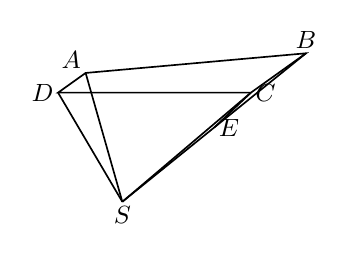
\begin{tikzpicture}[semithick, every node/.style={inner sep=1.4pt, font=\small}]
  \coordinate (D) at (0.000,0.000);
  \coordinate (C) at (2.449,0.000);
  \coordinate (A) at (0.350,0.250);
  \coordinate (B) at (3.149,0.500);
  \coordinate (S) at (0.816,-1.386);
  \coordinate (E) at (1.983,-0.443);

  % 底面
  \draw (A) -- (B) -- (C) -- (D) -- cycle;
  % 侧棱
  \draw (S) -- (D);
  \draw (S) -- (C);
  \draw (S) -- (A);
  \draw (S) -- (B);
  % CE
  \draw (C) -- (E);

  % 标注
  \node[left] at (D) {$D$};
  \node[right] at (C) {$C$};
  \node[above left] at (A) {$A$};
  \node[above] at (B) {$B$};
  \node[below] at (S) {$S$};
  \node[right] at (E) {$E$};
\end{tikzpicture}
\end{center}
\nopagebreak[4]
\Needspace{4\baselineskip}
\textbf{解析}

（1）设 $D(0,0,0)$，$CD$ 为 $x$ 轴，$AD$ 为 $y$ 轴，平面 $CSD$ 为 $xOz$ 平面。由 $AD=1$、$CS=2$、$CS\perp DS$ 及 $AS=\sqrt3$，解得 $CD=\sqrt6$，$S\left(\dfrac{\sqrt6}3,0,\dfrac2{\sqrt3}\right)$。由 $CE=\sqrt2$ 得 $BC=2$，$B(\sqrt6,2,0)$。

\Needspace{5\baselineskip}
平面 $BCS$ 的方程为 $x+\sqrt2z-\sqrt6=0$，故 $A(0,1,0)$ 到它的距离

\nopagebreak[4]
\[d=\frac{|0+0-\sqrt6|}{\sqrt3}=\sqrt2.\]

\Needspace{5\baselineskip}
（2）平面 $ACD$ 为 $z=0$，法向量 $(0,0,1)$。平面 $ECD$ 的法向量为 $(0,-1,\sqrt3)$，故

\nopagebreak[4]
\[\cos\theta=\frac{\sqrt3}{2},\qquad \theta=\frac\pi6.\]

\gkanswer{答案：（1）$\sqrt2$；（2）$\dfrac\pi6$。}

\end{answer}
\begin{answer}
\gksolhead{20}{}

\textbf{题目}：

已知以原点 $O$ 为中心的椭圆的一条准线方程为 $x=\dfrac{4\sqrt3}3$，离心率 $e=\dfrac{\sqrt3}2$，$M$ 是椭圆上的动点．

（1）若点 $C$，$D$ 的坐标分别是 $(0,-\sqrt3)$，$(0,\sqrt3)$，求 $|MC|\cdot|MD|$ 的最大值；

（2）如图，点 $A$ 的坐标为 $(1,0)$，$B$ 是圆 $x^2+y^2=1$ 上的点，$N$ 是点 $M$ 在 $x$ 轴上的射影，点 $Q$ 满足条件：$\overrightarrow{OQ}=\overrightarrow{OM}+\overrightarrow{ON}$，$\overrightarrow{QA}\cdot\overrightarrow{BA}=0$．求线段 $QB$ 的中点 $P$ 的轨迹方程．
\nopagebreak[4]
\begin{center}% 2009 年重庆卷理科第 20 题：椭圆 x^2+y^2/4=1、单位圆与点 A、B、M、N、Q。
% 来源 PDF：普通高考/2009/2009重庆理.pdf，SHA-256 6a815fa472e380a3f1143e8cdd93712e142309acb7a95176783499406a8e15f1。
% 原页：第 2 页（A3 三栏）第 2 栏中部，书页码 504。
% 重绘依据：按更正后的椭圆 x^2+y^2/4=1 绘制；取 M(0.8,1.2)、N(0.8,0)、Q(1.6,1.2)，
%   B 取单位圆上满足 QA⊥BA 的点 (-0.6,0.8)，仅作示意。
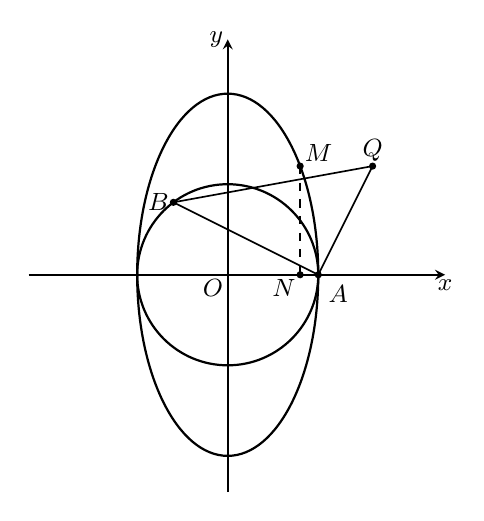
\begin{tikzpicture}[semithick, x=1.15cm, y=1.15cm, every node/.style={inner sep=1.4pt, font=\small}]
  % 坐标轴
  \draw[-stealth] (-2.2,0) -- (2.4,0) node[below] {$x$};
  \draw[-stealth] (0,-2.4) -- (0,2.6) node[left] {$y$};
  \node[below left] at (0,0) {$O$};

  % 椭圆
  \draw[thick] (0,0) ellipse (1 and 2);
  % 单位圆
  \draw[thick] (0,0) circle (1);

  % 点
  \coordinate (A) at (1.0,0.0);
  \coordinate (M) at (0.8,1.2);
  \coordinate (N) at (0.8,0.0);
  \coordinate (Q) at (1.6,1.2);
  \coordinate (B) at (-0.6,0.8);
  \fill (A) circle (1.3pt);
  \fill (M) circle (1.3pt);
  \fill (N) circle (1.3pt);
  \fill (Q) circle (1.3pt);
  \fill (B) circle (1.3pt);

  % 辅助线
  \draw[dashed] (M) -- (N);
  \draw (Q) -- (B);
  \draw (Q) -- (A);
  \draw (A) -- (B);

  % 标注
  \node[below right=2pt] at (A) {$A$};
  \node[above right] at (M) {$M$};
  \node[below left] at (N) {$N$};
  \node[above] at (Q) {$Q$};
  \node[left] at (B) {$B$};
\end{tikzpicture}
\end{center}
\nopagebreak[4]
\Needspace{4\baselineskip}
\textbf{解析}

\Needspace{5\baselineskip}
（1）按更正后的椭圆 $\dfrac{x^2}1+\dfrac{y^2}4=1$，$C(0,-\sqrt3)$、$D(0,\sqrt3)$ 为两焦点。设 $M(\cos\theta,2\sin\theta)$，则

\nopagebreak[4]
\[|MC|^2=4+3\sin^2\theta+4\sqrt3\sin\theta,\]
\nopagebreak[4]
\[|MD|^2=4+3\sin^2\theta-4\sqrt3\sin\theta.\]

\Needspace{5\baselineskip}
令 $u=\sin^2\theta$，则

\nopagebreak[4]
\[|MC|^2|MD|^2=(4+3u)^2-48u=(4-3u)^2.\]

故 $|MC||MD|=4-3u\leqslant4$，当 $u=0$（$M=(\pm1,0)$）取最大值 $4$。

\Needspace{5\baselineskip}
（2）设 $M(x_0,y_0)$，$N(x_0,0)$，$Q(2x_0,y_0)$；$B(u,v)$，$P(X,Y)$。由 $P$ 为 $QB$ 中点：

\nopagebreak[4]
\[x_0=X-\frac u2,\qquad y_0=2Y-v.\]

\Needspace{5\baselineskip}
$M$ 在椭圆上：

\nopagebreak[4]
\[\left(X-\frac u2\right)^2+\frac{(2Y-v)^2}{4}=1. \tag{1}\]

\Needspace{5\baselineskip}
又 $\overrightarrow{QA}\cdot\overrightarrow{BA}=0$：

\nopagebreak[4]
\[X(u-1)+Yv=0. \tag{2}\]

\Needspace{5\baselineskip}
由 (2) 与 $u^2+v^2=1$ 得

\nopagebreak[4]
\[u=\frac{X^2-Y^2}{X^2+Y^2},\qquad v=\frac{2XY}{X^2+Y^2}.\]

\Needspace{5\baselineskip}
代入 (1) 化简得

\nopagebreak[4]
\[4X^2-4X+4Y^2-3=0,\]

\Needspace{5\baselineskip}
即

\nopagebreak[4]
\[\left(X-\frac12\right)^2+Y^2=1.\]

\gkanswer{答案：（1）$4$；（2）$\left(x-\dfrac12\right)^2+y^2=1$。}

\end{answer}
\begin{answer}
\gksolhead{21}{}

\textbf{题目}：

设 $m$ 个不全相等的正数 $a_1,a_2,\cdots,a_m$（$m\geqslant7$）依次围成一个圆圈．

（1）若 $m=2009$，且 $a_1,a_2,\cdots,a_{1005}$ 是公差为 $d$ 的等差数列，而 $a_1,a_{2009},a_{2008},\cdots,a_{1006}$ 是公比为 $q=d$ 的等比数列；数列 $a_1,a_2,\cdots,a_m$ 的前 $n$ 项和 $S_n$（$n\leqslant m$）满足：$S_3=15$，$S_{2009}=S_{2007}+12a_1$，求通项 $a_n$（$n\leqslant m$）；

\Needspace{5\baselineskip}
（2）若每个数 $a_n$（$n\leqslant m$）是其左右相邻两数平方的等比中项，求证：

\nopagebreak[4]
\[a_1+\cdots+a_6+a_7^2+\cdots+a_m^2>ma_1a_2\cdots a_m.\]

\Needspace{4\baselineskip}
\textbf{解析}

\Needspace{5\baselineskip}
（1）设等比数列公比为 $q$。由 $S_{2009}-S_{2007}=a_{2008}+a_{2009}=12a_1$，且 $a_{2009}=a_1q$、$a_{2008}=a_1q^2$：

\nopagebreak[4]
\[q^2+q=12,\qquad q=3\ \text{\text{或}}\ q=-4.\]

\Needspace{5\baselineskip}
正数排除 $-4$，故 $q=3$。又题设公比 $q=d$，故 $d=3$。由 $S_3=15$：

\nopagebreak[4]
\[3a_1+3d=15,\qquad a_1+d=5,\qquad a_1=2.\]

\Needspace{5\baselineskip}
故 $1\leqslant n\leqslant1005$ 时

\nopagebreak[4]
\[a_n=2+3(n-1)=3n-1.\]

\Needspace{5\baselineskip}
后段 $a_1,a_{2009},a_{2008},\cdots,a_{1006}$ 为公比 $3$ 的等比数列，$a_{2009}=3a_1=6$，故

\nopagebreak[4]
\[a_n=6\cdot3^{2009-n}=2\cdot3^{2010-n}\qquad(1006\leqslant n\leqslant2009).\]

\Needspace{5\baselineskip}
（2）由 $a_n$ 是左右相邻两数平方的等比中项：

\nopagebreak[4]
\[a_n^2=a_{n-1}^2a_{n+1}^2,\]

\Needspace{5\baselineskip}
正数开方得 $a_n=a_{n-1}a_{n+1}$。于是

\nopagebreak[4]
\[\frac{a_{n+1}}{a_n}=\frac1{a_{n-1}},\]

\Needspace{5\baselineskip}
可推出 $a_{n+6}=a_n$，且六项之积为 $1$。将全部 $m$ 项相乘：

\nopagebreak[4]
\[\prod_{n=1}^m a_n=\prod a_{n-1}\prod a_{n+1}
=\left(\prod a_n\right)^2,\]

故 $\prod a_n=1$（正数）。

\Needspace{5\baselineskip}
由 $a_{n+6}=a_n$ 及 $m$ 为 $6$ 的倍数（绕圈一周后回到原值），设 $m=6k$，记 $S=a_1+\cdots+a_6$，$Q=a_1^2+\cdots+a_6^2$。则

\nopagebreak[4]
\[a_1+\cdots+a_6+a_7^2+\cdots+a_m^2=S+(k-1)Q.\]

\Needspace{5\baselineskip}
由均值不等式，$S\geqslant6\sqrt[6]{a_1\cdots a_6}=6$，$Q\geqslant6\sqrt[6]{a_1^2\cdots a_6^2}=6$。由于各数不全相等，至少一处严格，故

\nopagebreak[4]
\[S+(k-1)Q>6+6(k-1)=6k=m.\]

又 $\prod a_n=1$，即 $m a_1a_2\cdots a_m=m$，故原不等式成立。

\gkanswer{答案：（1）$1\leqslant n\leqslant1005$ 时 $a_n=3n-1$；$1006\leqslant n\leqslant2009$ 时 $a_n=2\cdot3^{2010-n}$；（2）证明见解析。}

\end{answer}